%           %experimenting with svn-multi

\svnkwsave{$RepoFile: siminos/froehlich/relStab.tex $}
\svnidlong {$HeadURL$}
{$LastChangedDate$}
{$LastChangedRevision$} {$LastChangedBy$}
\svnid{$Id$}


\section{Relative stability}
\label{sect:relStab}
%\PC{Write up here stability of relative solutions following \refref{DasBuch},
%\\
%\wwwcb{/chapters/continuous.pdf}
%    }

\subsection{\Reqva\ stability in a linear slice}

As an example of this we will calculate the stability matrix of a
relative equilibrium (\refdef{??}) in a slice.


\beq
{\MvarRed}(\sspRed)_{ij} = \Mvar(\sspRed)_{ij}-\velRel \cdot \Lg_{ij}
     -\groupTan(\sspRed)_i\,\left(
     \frac{\frac{\partial v}
     {\partial x_j}\cdot \groupTan(\sspRed)}{\braket{\groupTan(\sspRed)}{\sliceTan{}}}
     - \velRel \frac{\frac{\partial (\groupTan(\sspRed))}
              {\partial x_j}\cdot \sliceTan{}
              }{\braket{\groupTan(\sspRed)}{\sliceTan{}}}
              \right)
\ee{SF:redJacob1}


\subsection{\Reqva}

A \reqv\ is a trajectory that stays
within a group orbit of the symmetry group.

For a \reqv\ \REQV{}{} the flow and the group tangent vectors coincide, and
any point on the \reqv\ orbit is a fixed point in the co-moving frame,
a frame moving with velocity
     \toCB
\beq
\vel(\ssp) - \velRel \cdot \groupTan(\ssp) =0
    \,,\qquad
\ssp \in \pS_{\REQV{}{}}
\,.
\ee{SF:reqvTangent}
Dotting the equivariance condition \refeq{eq:InfnmslRot}, $ \groupTan_a(\vel)  - \Mvar(\ssp) \, \groupTan_a(\ssp) =0 $, by the velocity $c$, we get
\beq
( \Mvar -  \velRel \cdot \Lg) \vel =0
\,.
\ee{ReqvMargEig}
In other words, you have to be in the co-rotating
frame for eigenvalue to be marginal, and the velocity
be the corresponding right eigenvector.

In order for a trajectory to stay in the group orbit, its
velocity must always point in the tangent direction to the
group action, so we must have $\vel(\ssp) = \velRel(\tau)
\cdot \groupTan(\ssp)$ where $\velRel(\tau)_a$ is a scalar
function in terms of time.
    \PC{scalar? $\velRel(\tau)_a$ is an $N$-dimensional vector for
    $N$-dimensional group $\Group$. You are showing that
    for a compact Lie group $\velRel(\tau)_a = \velRel_a$ is constant
    independent of time, but the proof feels a bit clumsy.}
We also know that $x(\tau) = \LieEl(\tau) x(0)$ for some
element $\LieEl(\tau)$ of the symmetry group. Inserting this
into the first equation, we get that
\bea
\vel(\LieEl(\tau) \xInit) &=&
    \velRel(\tau)\cdot \groupTan(\LieEl(\tau) \xInit)
    \continue
\LieEl(\tau) \vel(\xInit) &=&
    \LieEl(\tau) \, \velRel(\tau) \cdot \groupTan(\xInit)
    \continue
\vel(\xInit) &=& \velRel(\tau) \cdot \groupTan(\xInit)
\eea
both $\vel(\xInit)$ and $\groupTan(\xInit)$ are independent of time, and we have $\velRel(\tau) = \velRel(0) = \velRel$ for all $\tau$, so $\velRel$ is an $N$-dimensional constant vector. If \SOn{n} is a rotational symmetry, $\velRel$ is called the `angular' velocity of the {\reqv}.

To further visualize the drifting of the flow around the
$z$-axis, we next find and plot the relative equilibria of
the \cLe. A {\reqv} is a solution of the flow which appears
stationary in a frame rotating at the appropriately chosen
constant angular velocity. We find these points in a manner
similar to finding the equilibria, with one difference. As
the flow drifts (rotates), a {\reqv} will drift as well, so
that instead of setting all of the $\vel(x)=0$, we allow the
component of $\vel(x)$ tangent to direction of group rotation to
be non-zero.

\subsection{Computing and plotting the {\reqv} $\REQB{1}$}

%                                              \exerbox{exer:CompRelEqu}
%                                              \exerbox{exer:PlotPolEqu}

Rebecca got for
$\REQB{1}$ in Cartesian coordinates
%                                             \exerbox{exer:PlotRelEqu}
\[\ssp_{\REQB{}1} = (8.48492,0.0771356,8.48562,0,26.9999)
\,,
\]
but I get (???).
\refFig{fig:CLERelEqui} shows the \cLf\ with initial point at
$\ssp_{\REQB{}1}$. The {\reqv} begins by tracing out a circle
around the $z$-axis, showing how the flow drifts. Eventually
numerical errors accumulate and the circle turns into a
``horn'' shape when the flow begins to spiral out.
%%%%%%%%%%%%%%%%%%%%%%%%%%%%%%%%%%%%%%%%%%%%%%%%%%%%%%%
% computed in equilibrium.nb
\begin{figure}[h]
\begin{center}
(a) % ~\includegraphics[width=0.35\textwidth]{CLERelEqui}
(b) % ~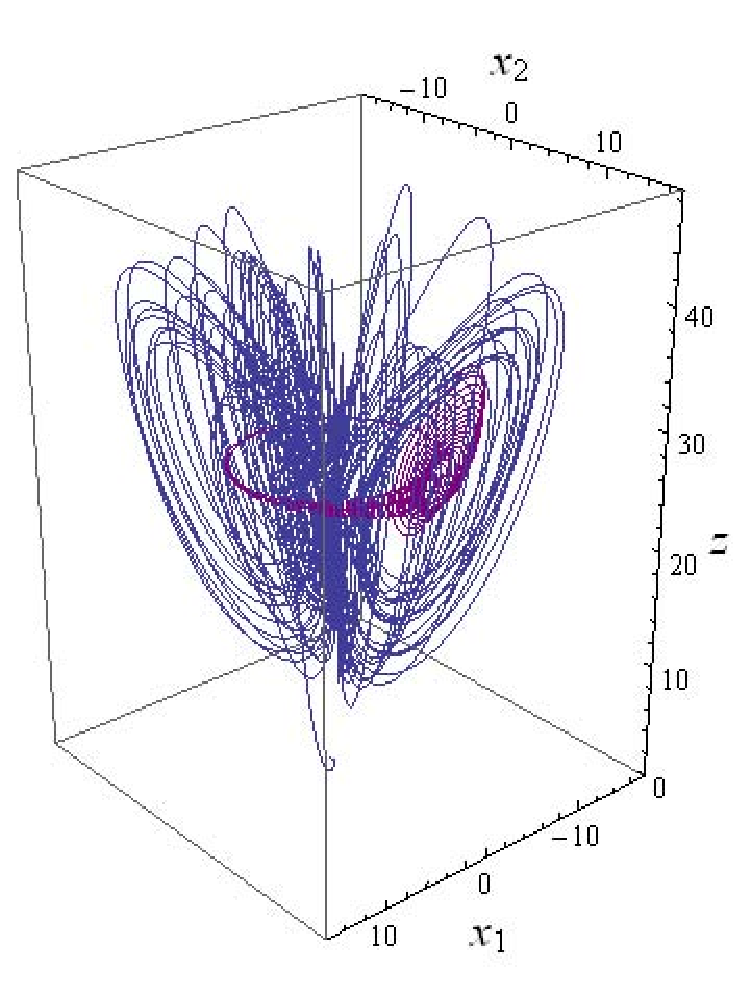
\includegraphics[width=0.35\textwidth]{CLEx1x2zRelEqu}
\end{center}
\caption{
Cartesian $\{x_1,x_2,z\}$ plot of the \cLf\ (a) with initial point
close to $\REQB{1}$, (b) superimposed over the strange attractor of
\reffig{fig:CLEx1x2z}.
    }
\label{fig:CLERelEqui}
\end{figure}
%%%%%%%%%%%%%%%%%%%%%%%%%%%%%%%%%%%%%%%%%%%%%%%%%%%%%%%

From here on, we examine the properties of the point defined above as
$\ssp_{\REQB{}1}$.

\subsection{Stability of \rpo s}
\label{SF:rpos}

In presence of a continuous symmetry we define the
\emph{{\FloquetM} for a \rpo} as the {\jacobianM} evaluated
at the period $\period{p}$ and rotated back into a \po\ by the
group action $\LieEl(\gSpace_p)$:
     \toCB
\beq
 \jMps_p(\ssp) = \LieEl(\gSpace_p)\jMps^\period{p}(\ssp)
    \,,\qquad
\ssp  \in \pS_p
\,.
\ee{SF:symPrimJac}
The argument of \refsect{sect:SFpos} goes through also in
the presence of a group rotation,
and \refeq{SF:transpEigPO} is correct for \rpo s as well.

% \subsection{Marginal eigenvalues}

The {\jacobianM} of a periodic orbit has marginal eigenvalues
when there is either a continuous symmetry (which can use to
reduce the problem) or a non-hyperbolicity in the flow (which
is not as easy to deal with).

To see that each continuous symmetry has a corresponding
marginal eigendirection, let $\ssp$ be any point on a periodic
orbit p with period $\period{p}$. If $\LieEl$ is any element in
the continuous symmetry Lie group $\Group$, then $f^t(\LieEl \ssp)
= \LieEl f^t(\ssp)$. By definition, $\jMps^t(\ssp)
\delta \ssp = \delta f^t(\ssp)$.
Close to identity $\LieEl = 1+\delta
\theta \cdot \Lg$ is an infinitesimal Lie group element and
$\delta \ssp = \ssp - \LieEl \ssp = \ssp - (1+\delta \theta
\cdot \Lg) \ssp  = \delta \theta \cdot \Lg \ssp,$
so
$\delta f^{\period{p}}(\ssp) = f^{\period{p}}(\ssp) -
f^{\period{p}}(\LieEl \ssp)= f^{\period{p}}(\ssp) - \LieEl f^{\period{p}}(\ssp) =
\ssp - \LieEl \ssp = \delta \theta \cdot \Lg \ssp$.
This gives us
$\jMps_p(\ssp) \delta \theta \cdot \Lg \ssp = \delta
\theta \cdot \Lg \ssp$,
\ie, a set of marginal direction eigenvectors
\beq
 \jMps_p(\ssp) \groupTan_{a}(\ssp) =
\groupTan_{a}(\ssp)
\ee{SF:symMargEig}
with unit eigenvalues $\ExpaEig_a=1$,
where $\groupTan_{a}(\ssp)$ is a group tangent \refeq{PC:groupTan}.
    \PC{prove this for a \rpo, using definition \refeq{SF:symPrimJac};
        the \po\ marginal eigenvalue should be a special case.}


\subsection{Stability of \reqva\ in \reducedsp}
%SF June 22 2010

Using the parameters \refeq{SiminosPrmts}, we get the
 $\REQB{1}$ stability eigenvalues
\[
0.0938 \pm 10.1945i,-22.0000,-13.8534,-11.009
\]
with corresponding eigenvectors
        \PC{ChaosBook convention is to order eigenvalues
        from most positive (unstable) to the most negative.
        \\
        Replace complex eigenvectors by the real,
        imaginary parts, as that is what you actually use - I
        did this in \refeq{eigVecQ1}.
        }
\bea
&&(0.3378\mp 0.3411i,0.6887,0.0017\mp 0.0031i,0.5133\mp 0.1706i,-0.0029\mp 0.0511i)
\continue
&&(0.9939,0.0470,0.0009,-0.0994,0.0051)
\continue
&&(-0.8966,0.3457,0.0097,-0.2755,0.0246)
\continue
&&(0.0210,-0.0203,-0.995,0.0095,-0.0011)
\nnu
\eea
These are the same as the eigenvalues found using polar coordinates with the addition of $-22.0000$.
    \PC{
    ``the addition of $-22.0000$'' means what?
    }

The equations of motion for trajectory kept in a hyperplane by rotation under the symmetry group are:
\bea
    \dot{\gSpace}_a (\sspRed) &=&
    \frac{\braket{\vel(\sspRed)}{\sliceTan{a}}}
         {\braket{\groupTan(\sspRed)}{\sliceTan{}}}
    \continue
    u(\sspRed) &=& \vel(\sspRed)-\dot{\gSpace}(\sspRed)  \cdot \groupTan(\sspRed)
\eea
where $\vel(\sspRed)$ is the velocity of the full \statesp\ flow, $\groupTan(\sspRed)$ is the tangent to the group action, and $\sliceTan{}$ is the vector normal to the hyperplane of the slice. Using this equation we get that the {\stabmat} $\MvarRed$ for the system in \reducedsp\ is given by:
    \PC{Stefan's version was
\[
M_{ij} =
A_{ij}-c I_{ij} -(Tx)_i\,(\frac{\frac{\partial v}{\partial x_i}\cdot \sliceTan{}}
        {Tx \cdot \sliceTan{}}
      - c \frac{\frac{\partial (Tx)}{\partial x_j}\cdot \sliceTan{}}{Tx \cdot \sliceTan{}})
\]
    hopefully no errors introduced in my rewrite
    }
\beq
{\MvarRed}(\sspRed)_{ij} = \Mvar(\sspRed)_{ij}-\velRel \cdot \Lg_{ij}
     -\groupTan(\sspRed)_i\,\left(
     \frac{\frac{\partial v}
     {\partial x_j}\cdot \sspRed}{\braket{\groupTan(\sspRed)}{\sliceTan{}}}
     - \velRel \frac{\frac{\partial (\groupTan(\sspRed))}
              {\partial x_j}\cdot \sliceTan{}
              }{\braket{\groupTan(\sspRed)}{\sliceTan{}}}
              \right)
\ee{SF:redJacob2}

                                                    \exerbox{exer:Reducedstab}


\subsection{Eigen-system of the slice \stabmat}

As in \refsect{sect:stability}, we now find and plot the
eigen-system of the \stabmat\ in order to understand the
stability of $\REQB{1}$.
Rebecca finds the eigenvalues
\beq
(\lambda_{1,2},\lambda_3,\lambda_4)
= (0.0938179 \pm 10.1945 i,-11.0009,-13.8534)
\ee{RW:REQB1eigvals}
with the eigenvectors
\bea
\Re e_{1} &=& \Re e_{2} = (-0.266121, -0.0321133, 0.00034139, 0.719222)
\continue
\Im e_{1}  &=& -\Im e_{2} = (-0.295017, 0.569063, -0.000551886,0)
\continue
e_3 &=& (-0.0883591, -0.0851485, -0.989135, -0.0809553)
\continue
e_4 &=& (-0.855586, -0.329912, -0.00273531, -0.398902)
\,.
\label{eigVecQ1}
\eea

As in \refsect{sect:stability}, we can also plot the flow
with an initial point very near to
$\REQB{1}$ along one of the eigenvectors.
% \refFig{fig:CLEQ1} shows just this.
                                                    \exerbox{exer:EigenQ1}
                                                    \exerbox{exer:PlotPolEigenQ1}

    \PublicPrivate{}{
\subsection{\Rpo\ stability in \reducedsp}

    \PC{Stefan, please write up your ``three programs for approximating
    the \jacobianM\ along any trajectory.'' Derive here \rpo\
    {\monodromyM} in the \reducedsp, test it on some of the Evangelos
    \rpo s for \cLe. }

    } %end     \PublicPrivate{}{
